
% Lab1 for ENGR 1120 030 130 - Tristan Hill - Spring 2016 - Summer 2017 - Fall 2017 - Spring 2018 - Summer 2018 - Sprin 2020
% 
% Introduction to MATLAB 
%
% Variables - Assigning - Accessing - Overwriting - Incrementing
% Basic User Input and Output 
 

% Document settings
\documentclass[11pt]{article}
\usepackage[margin=1in]{geometry}
\usepackage[pdftex]{graphicx}
%\graphicspath{{images/}} %Setting the graphicspath

\usepackage{multirow}
\usepackage{setspace}
\usepackage{hyperref}
\usepackage{color,soul}
\usepackage{fancyvrb}
\usepackage{framed}
\usepackage{wasysym}
\usepackage{multicol}

\pagestyle{plain}
\setlength\parindent{0pt}
\hypersetup{
    bookmarks=true,         % show bookmarks bar?
    unicode=false,          % non-Latin characters in Acrobat’s bookmarks
    pdftoolbar=true,        % show Acrobat’s toolbar?
    pdfmenubar=true,        % show Acrobat’s menu?
    pdffitwindow=false,     % window fit to page when opened
    pdfstartview={FitH},    % fits the width of the page to the window
    pdftitle={My title},    % title
    pdfauthor={Author},     % author
    pdfsubject={Subject},   % subject of the document
    pdfcreator={Creator},   % creator of the document
    pdfproducer={Producer}, % producer of the document
    pdfkeywords={keyword1} {key2} {key3}, % list of keywords
    pdfnewwindow=true,      % links in new window
    colorlinks=true,       % false: boxed links; true: colored links
    linkcolor=red,          % color of internal links (change box color with linkbordercolor)
    citecolor=green,        % color of links to bibliography
    filecolor=magenta,      % color of file links
    urlcolor=blue           % color of external links
}

% assignment number 
\newcommand{\NUM}{1} 
\newcommand{\VSpaceSize}{2mm} 
\newcommand{\HSpaceSize}{2mm} 

\newcommand{\secNum}{GSET: Programming}
\newcommand{\assnType}{Lab}
\newcommand{\assnTitle}{Variables and Assignment}
\newcommand{\assnNum}{1} 
\newcommand{\currTerm}{Summer 2022}

\definecolor{mygray}{rgb}{.6, .6, .6}

\setulcolor{red} 
\setstcolor{green} 
\sethlcolor{mygray} 

\begin{document}

	\textbf{\LARGE \secNum \hspace{1mm} - \hspace{1mm} \currTerm} \\\\
	\textbf{\LARGE \assnType \hspace{1mm}  \assnNum : \assnTitle} \\\\
	\textbf{Names:\underline{\hspace{140mm}} } \\
	\begin{description}

		\item [\textbf{ \large Overview}] \textbf{ \Large :}\\
			You will learn to use variables to store decimal numbers and practice a few basic calculations with the MATLAB command syntax. Turn in this sheet with the answers and a record of the commands you used to solve each problem.

        \item [\textbf{ \large Assignment}] \textbf{ \Large :}
            \begin{enumerate}
            \item ($\frac{40}{100}$ pts.)
            Assume the {\bf shape 1} and {\bf shape 2} below are made of steel with a density of 8050 $\frac{kg}{m^3}$. Use the command window to calculate the {\it mass} of {\bf shape 1} shown below.\\
            
            	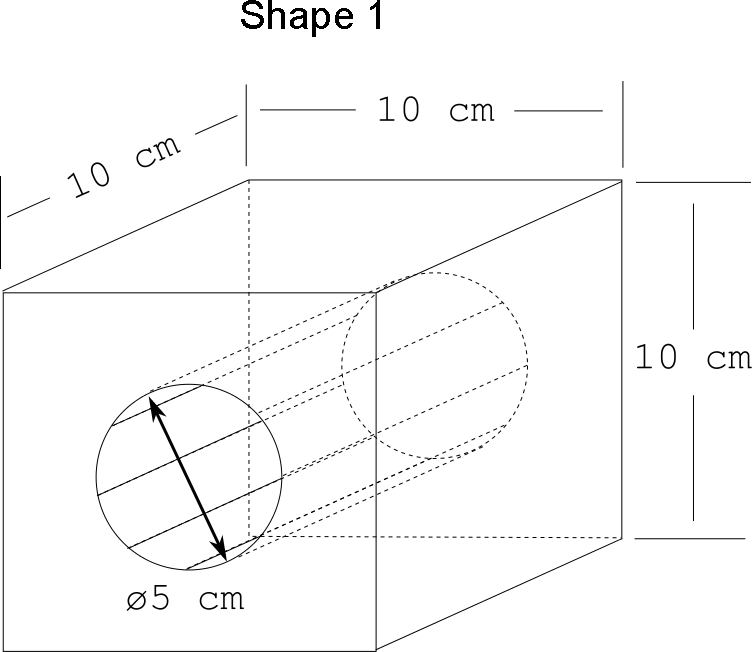
\includegraphics[scale=.25]{images/lab1_fig1.png}\\
               
\underline{\hspace{140mm}}\\\\
\underline{\hspace{140mm}}\\\\
\underline{\hspace{140mm}}\\\\

{\textbf volume: \underline{\hspace{60mm}}}\\

\underline{\hspace{140mm}}\\\\
\underline{\hspace{140mm}}\\\\
\underline{\hspace{140mm}}\\\\		
	
{\textbf mass: \underline{\hspace{60mm}}}\\
	
            \item ($\frac{40}{100}$ pts.)
             Use the command window to calculate the {\it mass} of {\bf shape 2} shown below. \\
            
            	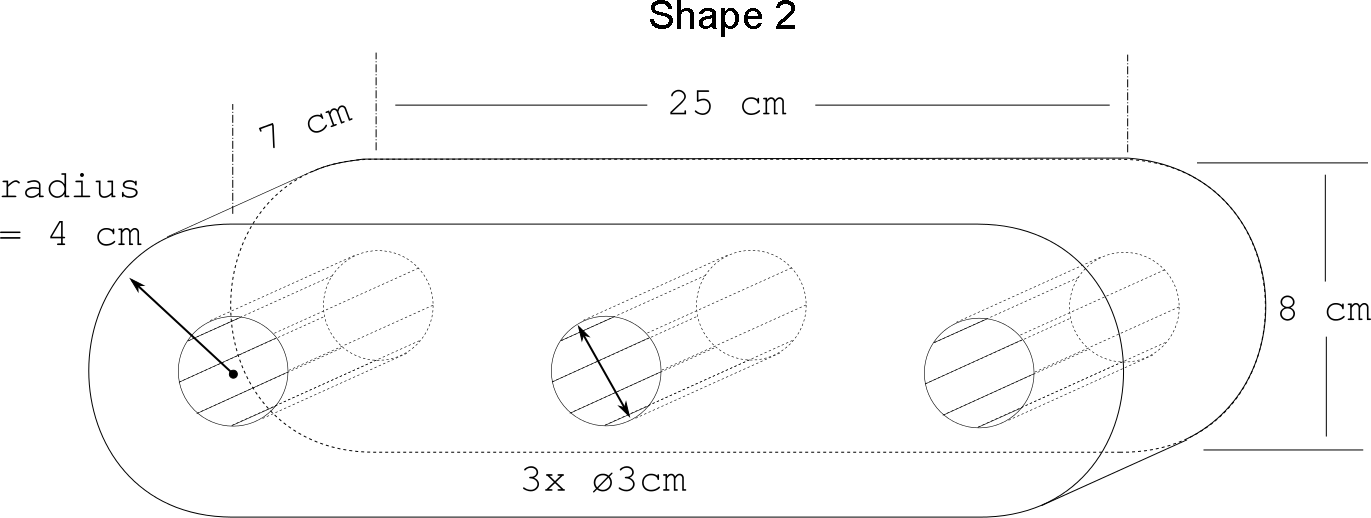
\includegraphics[scale=.25]{images/lab1_fig2.png}
		\vspace{5mm}\\
\underline{\hspace{140mm}}\\\\
\underline{\hspace{140mm}}\\\\
\underline{\hspace{140mm}}\\\\
\underline{\hspace{140mm}}\\\\
\underline{\hspace{140mm}}\\\\
\underline{\hspace{140mm}}\\\\
{\textbf volume: \underline{\hspace{60mm}}}\\
\underline{\hspace{140mm}}\\\\
\underline{\hspace{140mm}}\\\\
\underline{\hspace{140mm}}\\\\
\underline{\hspace{140mm}}\\\\
\underline{\hspace{140mm}}\\\\
\underline{\hspace{140mm}}\\\\		
	
{\textbf mass: \underline{\hspace{60mm}}}\\

\newpage	
            \item ($\frac{20}{100}$ pts.) Imagine you are an engineer designing {\bf shape 1}. Your job is to reduce the mass of {\bf shape 1} to exactly 5 kg. You must do this by increasing the size of the hole. What is the diameter of the hole that would make the mass equal to exactly 5 kg?\\
		\vspace{5mm}\\
		diameter: \underline{\hspace{50mm}}
        	\end{enumerate}

\underline{\hspace{140mm}}\\\\
\underline{\hspace{140mm}}\\\\
\underline{\hspace{140mm}}\\\\
\underline{\hspace{140mm}}\\\\
\underline{\hspace{140mm}}\\\\
\underline{\hspace{140mm}}\\\\
\underline{\hspace{140mm}}\\\\
\underline{\hspace{140mm}}\\\\
\underline{\hspace{140mm}}\\\\
\underline{\hspace{140mm}}\\\\
\underline{\hspace{140mm}}\\\\
\underline{\hspace{140mm}}\\\\
\underline{\hspace{140mm}}\\\\			
\underline{\hspace{140mm}}\\\\
\underline{\hspace{140mm}}\\\\	    
\newpage
\underline{\hspace{140mm}}\\\\
\underline{\hspace{140mm}}\\\\
\underline{\hspace{140mm}}\\\\
\underline{\hspace{140mm}}\\\\
\underline{\hspace{140mm}}\\\\
\underline{\hspace{140mm}}\\\\
\underline{\hspace{140mm}}\\\\
\underline{\hspace{140mm}}\\\\
\underline{\hspace{140mm}}\\\\
\underline{\hspace{140mm}}\\\\
\underline{\hspace{140mm}}\\\\
\underline{\hspace{140mm}}\\\\
\underline{\hspace{140mm}}\\\\			
\underline{\hspace{140mm}}\\\\
\underline{\hspace{140mm}}\\\\	 
\underline{\hspace{140mm}}\\\\
\underline{\hspace{140mm}}\\\\			
\underline{\hspace{140mm}}\\\\
\underline{\hspace{140mm}}\\\\	 

%\newpage
%\item [\textbf{ \large Geometry Puzzle}] \textbf{ \Large :}\\
%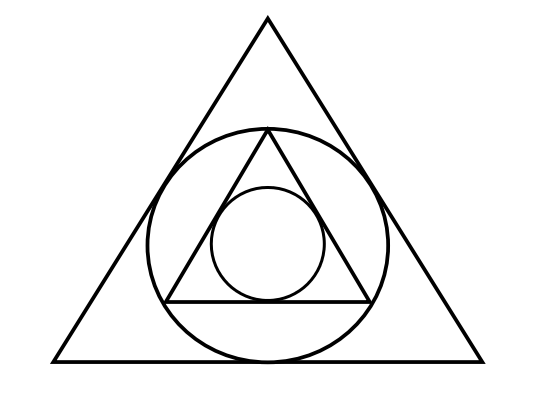
\includegraphics[scale=0.7]{triangle_puzzle.png}	\\
%
%\Large {\bf What is the ratio of the volume of the small triangle to volume of the large triangle?}\\\\\\\\
%\Large {\bf What is the ratio of the volume of the small circle to volume of the large circle?}\\\\\\\\
%\Large {\bf How can you prove it?}
\end{description}
 
\end{document}



